% Nama Kelompok : Kelompok 3
% Kelas : D4 TI 1A
% 1. Kadek Diva Krishna Murti (1174006)
% 2. Niko
% 3. Rizal Rony Sitorus
% 4. Jeremia
% 5. Sri Rahayu (1174015)

\begin{figure}[ht]
\centerline{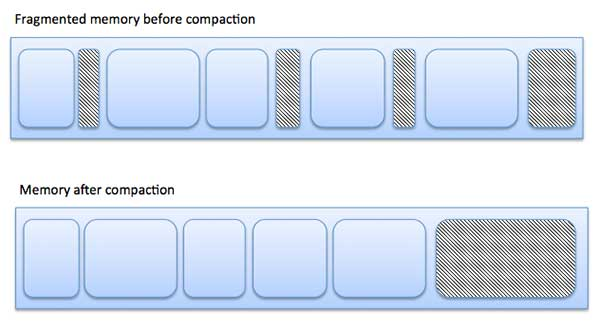
\includegraphics[width=1\textwidth]{figures/fragmentation.jpg}}
\caption{Contoh fragmentasi.}
\label{fragmentasi}
\end{figure}

\section{Definisi Fragmentasi}
Fragmentasi \ref{fragmentasi} adalah sebuah fenomena di ruang penyimpanan yang digunakan secara tidak efisien, mengurangi kapasitas penyimpanan. Istilah ini juga digunakan untuk menunjukkan tempat yang gersang itu sendiri. Dapat disimpulkan bahwa fragmentasi adalah munculnya lubang-lubang yang tidak cukup besar untuk menampung permintaan dari proses.

\section{Jenis-Jenis Fragmentasi}
Fragmentasi dapat berupa fragmentasi internal maupun fragmentasi eksternal.
\subsection{Fragmentasi Internal}
Berdasarkan buku yang berjudul Sistem Operasi \cite{pangera2005sistem} fragmentasi internal adalah tidak efisiennya utilitas memori utama di mana sembarang program sekecil apapun tidak bergantung, akan menempati seluruh partisi. Keadaan ini mengakibatkan pemborosan ruang yang bersifat internal terhadap partisi dengan kenyataan di mana blok data yang dimuatkan berukuran lebih kecil dari partisi.

Fragmentasi internal terjadi pada saat di mana jumlah memori yang diberikan oleh penjadwal CPU untuk ditempati proses lebih besar dari pada yang diminta oleh proses karena adanya selisih antara permintaan proses dengan alokasi lubang yang sudah ditetapkan tetapi untuk satu partisi tertentu hanya berukuran kecil sehingga tidak digunakan.
Hal ini umumnya terjadi ketika kita menggunakan sistem partisi banyak tetap. Kembali ke contoh sebelumnya, di mana ada proses dengan permintaan memori sebesar 17 KB dan memori dipartisi menjadi blok yang masing-masing besarnya 5 KB. Pada sistem partisi banyak tetap, memori yang dialokasikan untuk proses adalah 4 blok, atau sebesar 20 KB. Padahal, yang terpakai hanya 17 KB. Sisa 3 KB tetap diberikan pada proses tersebut, walaupun tidak dipakai oleh proses tersebut. Hal ini berarti pula proses lain tidak dapat memakainya. Perbedaan memori yang dialokasikan dengan yang diminta inilah yang disebut fragmentasi internal. Pada multiple partition, fragmentasi internal mungkin terjadi pada situasi berikut. Misalnya terdapat lubang 18464 byte, dan proses meminta 18462 byte seperti pada Gambar \ref{fragmentasiinternal}. Alokasi dilakukan sesuai permintaan maka sisa lubang 2 byte. Penyimpanan lubang ini akan memerlukan memori lebih besar dari lubang itu sendiri. Pendekatannya adalah dengan mengalokasikan lubang yang sangat kecil sebagai bagian dari permintaan yang besar.

Fragmentasi internal tidak dapat dihindarkan apabila kita menggunakan sistem partisi banyak berukuran tetap, mengingat besar lubang – lubang yang disediakan selalu tetap, kecuali jika kita menggunakan sistem partisi banyak dinamis, yang memungkinkan suatu proses untuk diberikan ruang memori sebesar yang dia minta.

\subsection{Fragmentasi Eksternal}
Berdasarkan buku yang berjudul Sistem Operasi \cite{pangera2005sistem} fragmentasi eksternal adalah keadaan di mana suatu proses pada awalnya berjalan dan bekerja dengan baik, namun ketika mengarah ke situasi yang di mana terdapat banyak lubang - lubang kecil di dalam sebuah memori sehingga semakin lama memori tersebut semakin terfragmentasi dan utilisasi memori pun kinerjanya menjadi menurun sehubungan dengan kenyataan bahwa memori bersifat eksternal terhadap semua partisi menjadi sangat terfragmentasi. Keadaan ini merupakan kebalikan dari fragmentasi ini.

Fragmentasi eksternal terjadi pada saat di mana jumlah keseluruhan memori kosong yang tersedia memang mencukupi untuk menampung permintaan tempat dari proses, tetapi tidak dapat dialokasikan karena letaknya tidak berkesinambungan atau tidak berurutan atau terpecah menjadi beberapa bagian kecil sehingga proses tidak dapat masuk. 
Umumnya, ini terjadi ketika kita menggunakan sistem partisi banyak dinamis. Pada sistem partisi banyak dinamis, seperti yang diungkapkan sebelumnya, sistem terbagi menjadi blok-blok yang besarnya tidak tetap. Maksud tidak tetap di sini adalah blok tersebut bisa bertambah besar atau bertambah kecil. 

Misalnya sebuah proses meminta ruang memori sebesar 17KB, sedangkan memori dipartisi menjadi blok-blok yang besarnya masing-masing 5 KB. Maka yang akan diberikan proses adalah 3 blok ditambah 2 KB dari sebuah blok. Sisa blok yang besarnya 3 KB akan disiapkan untuk menampung proses lain atau jika ia bertentangga dengan ruang memori yang kosong, ia akan bergabung dengannya. Akibatnya dengan sistem partisi banyak dinamis, bisa tercipta lubang-lubang di memori, yaitu ruang memori yang kosong. Keadaan saat lubang-lubang ini tersebar yang masing-masing lubang tersebut tidak ada yang bisa memenuhi kebutuhan proses padahal jumlah dari besarnya lubang tersebut cukup untuk memenuhi kebutuhan proses disebut sebagai fragmentasi eksternal. Fragmentasi eksternal dilakukan pada algoritma alokasi dinamis, terutama strategi first-fit dan best-fit.

Fragmentasi eksternal dapat diatasi dengan beberapa cara, diantaranya adalah :

\begin{enumerate}

\item Compaction atau Pemadatan\\
Compaction atau Pemadatan, yaitu memadatkan atau mengatur kembali isi memori agar memori yang kosong diletakkan bersama di suatu bagian yang besar sehingga proses dapat masuk ke ruang memori kosong tersebut. Pemadatan hanya dapat dilakukan apabila relokasi bersifat dinamis dan pengalamatan program dilakukan pada saat program dieksekusi. Kebutuhan akan pemadatan akan hilang bila pengalamatan dapat dilakukan secara berurutan, walaupun sebenarnya proses tidak ditempatkan pada lokasi memori yang berurutan. Nantinya, konsep ini diterapkan dengan Paging. Pemadatan tidak selalu dapat dipakai. Agar proses dapat dieksekusi pada lokasi baru, semua alamat internal harus direlokasi.
Pemadatan hanya dilakukan pada relokasi dinamis dan dikerjakan pada waktu eksekusi. Karena relokasi membutuhkan pemindahan program dan data dan kemudian mengubah register basis (atau relokasi) yang mencerminkan alamat basis baru. Terdapat beberapa cara pemadatan seperti pada Gambar \ref{pemadatan}.

\begin{figure}[ht]
\centerline{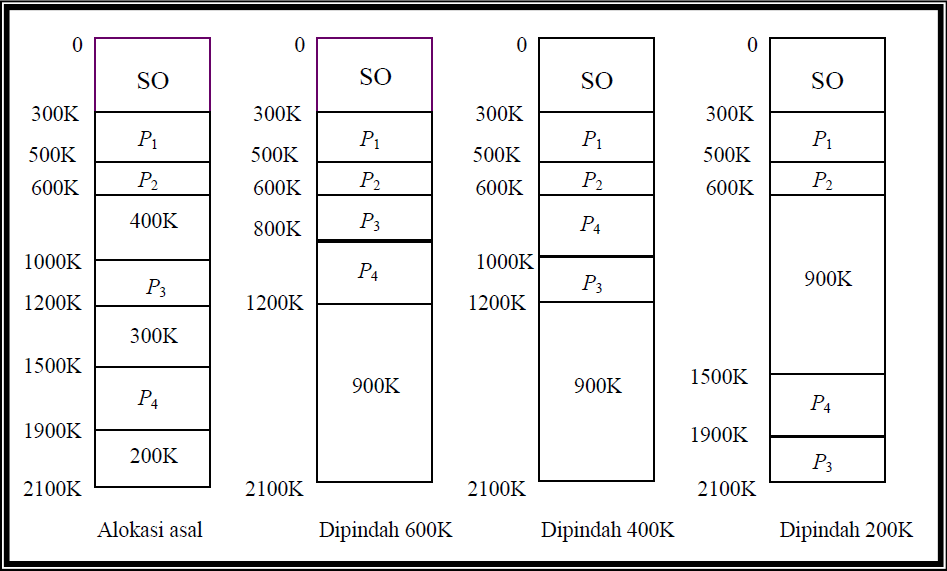
\includegraphics[width=1\textwidth]{figures/pemadatan.png}}
\caption{Compaction atau Pemadatan.}
\label{pemadatan}
\end{figure}


\item Penghalaman atau Paging \\
Penghalaman atau paging  merupakan metode yang memungkinkan suatu alamat fisik memori yang tersedia dapat tidak berurutan. Pemberian halaman bisa menjadi solusi untuk pemecahan masalah luar. Untuk bisa mengimplementasikan solusi ini adalah melalui pengunaan dari skema pemberian halaman. Dengan pemberian halaman bisa mencegah masalah penting dari pemuatan besar ukuran memori yang bervariasi kedalam penyimpanan cadangan. Ketika beberapa pecahan kode dari data yang tersisa di memori utama perlu untuk ditukar keluar, harus ditemukan ruang untuk penyimpanan cadangan. Masalah pemecahan kode didiskusikan dengan kaitan bahwa pengaksesannya lebih lambat. Biasanya bagian yang menunjang untuk pemberian halaman telah ditangani oleh perangkat keras. Bagaimana pun, desain yang ada baru-baru ini telah diimplementasikan dengan menggabungkan perangkat keras dan sistem operasi, terutama pada microprocessor 64 bit.

\item Segmentasi\\
Segmentasi merupakan skema manajemen memori yang mendukung cara pandang seorang programmer terhadap memori. Ruang alamat logika merupakan sekumpulan dari segmen-segmen. Masing-masing segment mempunyai panjang dan nama. Alamat diartikan sebagai nama segmen dan offset dalam suatu segmen. Jadi jika seorang pengguna ingin menunjuk sebuah alamat dapat dilakukan dengan menunjuk nama segmen dan offsetnya. Untuk lebih menyederhanakan implementasi, segmen-segmen diberi nomor yang digunakan sebagai pengganti nama segment. Sehingga, alamat logika terdiri dari dua tupple: [segment-number, offset].

\end{enumerate}

\begin{figure}[ht]
\centerline{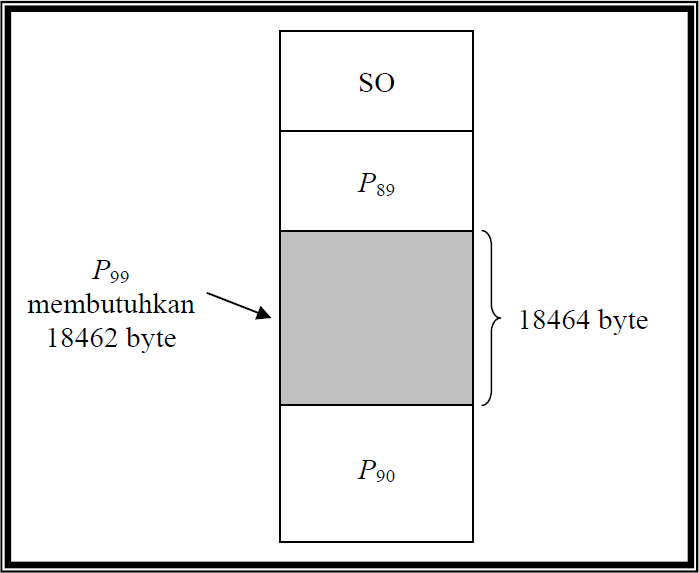
\includegraphics[width=1\textwidth]{figures/fragmentasi_internal.png}}
\caption{Fragmentasi Internal.}
\label{fragmentasiinternal}
\end{figure}

\subsection{Fragmentasi Data}

Data fragmentasi terjadi ketika sebuah bagian dari data dalam memori rusak ke dalam banyak potongan-potongan yang tidak saling berdekatan. Hal ini biasanya hasil dari mencoba untuk memasukkan benda yang besar ke dalam penyimpanan yang telah menderita fragmentasi eksternal.

Misalnya, file dalam file sistem biasanya diatur dalam unit yang disebut blok atau kelompok. Ketika sebuah file sistem yang dibuat, ada ruang untuk menyimpan file blok bersama contiguously. Hal ini memungkinkan untuk cepat berurut membaca dan menulis file. Namun, seperti file ditambahkan, dihapus, dan berubah dalam ukuran, ruang bagi menjadi eksternal, hanya meninggalkan lubang kecil di tempat yang tepat untuk data baru. Bila file yang baru ditulis, atau jika file yang sudah ada diperpanjang, maka data baru blok pasti tersebar, karena perlambatan akses untuk mencari waktu dan pemutaran penundaan dari membaca / menulis head, dan overhead incurring tambahan untuk mengelola tambahan lokasi. Hal ini disebut fragmentasi file system.

Sebagai contoh lain, jika node yang terhubung daftar dialokasikan turut dalam memori, ini akan meningkatkan lokalitas dari referensi dan data cache meningkatkan kinerja selama traversal dari daftar. Jika memori renang gratis bagi ruang adalah, baru node akan tersebar di seluruh memori, meningkatkan jumlah cache misses.

Seperti compaction dapat menghilangkan fragmentasi eksternal, data fragmentasi dapat dihapuskan oleh rearranging data terkait agar buah yang saling berdekatan. Misalnya, pekerjaan utama dari defragmentation alat ini untuk mengatur ulang blok pada disk, sehingga setiap file blok yang berdekatan. Paling defragmenting utilitas juga berusaha untuk mengurangi atau menghilangkan fragmentasi ruang kosong. Beberapa pindah pengumpul sampah terkait juga akan memindahkan objek dekat bersama (disebut Memadatkan) untuk meningkatkan kinerja cache.

\section{Kesimpulan}

Algoritma alokasi penyimpanan dinamis mana pun yang digunakan, tetap tidak bisa menutup kemungkinan terjadinya fragmentasi. Bahkan hal ini bisa menjadi fatal. Salah satu kondisi terburuk adalah apabila kita memiliki memori terbuang setiap dua proses. Apabila semua memori terbuang itu digabungkan, bukan tidak mungkin akan cukup untuk menampung sebuah proses. Sebuah contoh statistik menunjukkan bahwa saat menggunakan metoda first fit, bahkan setelah dioptimisasi, dari N blok teralokasi, sebanyak 0.5N blok lain akan terbuang karena fragmentasi. Jumlah sebanyak itu berarti kurang lebih setengah dari memori tidak dapat digunakan. Hal ini disebut dengan aturan 50\%.
\\
\\
Beberapa jenis strategi pencocokan antara lain:
\begin{table}[h!]
\centering
\begin{tabular}{ |c|c|l| }
\hline
1 & Cocok pertama (first fit) & Pencocokan terjadi menurut antrian informasi \\
\hline
2 & Cocok pertama berdaur (cyclical first fit) &  Pencocokan tidak harus dimulai dari urutan penggalan memori yang pertama, tetapi dapat dilakukan setelah terjadi pencocokan sebelumnya. \\
\hline
3 & Cocok terbaik (best fit) &  Pencocokan dilakukan sesuai dengan penggalan memori yang ukurannya pas. \\
\hline
4 & Cocok terburuk (Worst fit) & Informasi akan menempati penggalan yang ukurannya terbesar. \\
\hline
\end{tabular}
\end{table}
